\section{Multiprocesinės operacinės sistemos modelis}

\subsection{Procesai}

Procesas - tai atskira vykdoma programa, kartu su esamomis registrų reikšmėmis ir savo kintamaisiais.
Kiekvienam procesui yra sukuriamas atskiras virtualus procesorius. Programa nuo proceso skiriasi tuo, kad procesas yra kokioje nors veikimo stadijoje esanti programa,
o programa - tam tikras baitų rinkinys. Proceso veikimo stadiją apibūdina proceso deskriptorius. Jame laikomi visi procesui reikalingi parametrai.\\

\subsubsection{Deskriptoriai}
Deskriptoriai yra dinaminiai objektai, kurie gali būsi sukurti ir sunaikinti sistemos veikimo metu. Procesus kuria procesai, todėl turi egzistuoti vienas pagrindinis procesas, 
kuriantis visus kitus.\\

Procesų deskriptoriai:
	\begin{itemize}
		\item PD - proceso vidinis vardas
		\item PID - proceso išorinis vardas
		\item PCPU - proceso būsena ir teisės
		\item PChild - proceso vaikų ID
		\item PParent - proceso tėvo ID
		\item PPriority - proceso prioritetas 0 - 100
		\item PRes - proceso sukurti resursai
		\item PRecRes - proceso kūrimo metu perduoti resursai
		\item PList - procesų sąrašas, kuriam priklauso procesas
	\end{itemize}

Procesus galima suskirstyti į:
	\begin{itemize}
		\item Vartotojiškus - vykdančius vartotojo programą
		\item Sisteminius - aptarnaujančius vartotojiškus.
	\end{itemize}

Procesas gauna procesorių tik tada, kai jam netrūksta jokio kito resurso ir tampa vykdomu. Tokioje būsenoje procesas išlieka tol, kol sistemoje neįvyksta pertraukimas 
arba einamasis procesas nepaprašo kokio nors resurso. Jei procesas nereikalauja jokio resurso, iš jo gali būti atimtas procesorius, nes per ilgai dirbo.\\
Procesų būsenos:
	\begin{itemize}
		\item Vykdomas - turi procesorių
		\item Blokuotas - prašo resurso (išskyrus procesorių)
		\item Pasiruošęs - vienintelis trūkstamas resursas yra procesorius
		\item Sustabdytas - kito proceso sustabdytas procesas
	\end{itemize}

Diagrama, vaizduojanti, kaip procesas gali pakliūti i tam tikrą būseną ir iš jos išeiti:

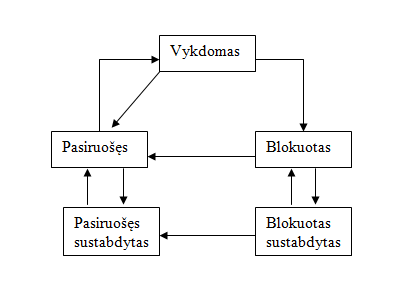
\includegraphics{img/processDiagram.png}

	\begin{itemize}
		\item Vykdomas procesas blokuojasi jam prašant ir negavus resurso.
		\item Vykdomas procesas tampa pasiruošusiu atėmus iš jo procesorių dėl kokios nors priežasties
		\item Blokuotas procesas tampa pasiruošusiu, kai yra suteikiamas reikalingas resursas.
		\item Pasiruošę procesai varžosi dėl procesoriaus. Gavęs procesorių procesas tampa vykdomu.
		\item Procesas gali tapti sustabdytu blokuotu, jei einamasis procesas jį sustabdo, kai jis jau ir taip jau yra blokuotas
		\item Procesas tampa blokuotu iš blokuoto sustabdyto, jei einamasis procesas nuima būseną sustabdytas.
		\item Procesas gali tapti pasiruošusiu sustabdytu, jei einamasis procesas jį sustabdo, kai jis yra pasiruošęs.
		\item Procesas tampa pasiruošusiu iš pasiruošusio sustabdyto, jei einamasis procesas nuima būseną sustabdytas.
		\item Procesas tampa pasiruošusiu iš blokuoto sustabdyto, jei procesui yra suteikiamas jam reikalingas resursas.
	\end{itemize}

\subsubsection{Procesų planuotojas}
Procesų planuotojo paskirtis - atimti procesorių iš proceso, peržvelgti pasiruošusių procesų sąrašą, išrinkti iš jo tinkamiausią procesą ir jam perduoti procesorių.
Planuotojas turi įgyvendinti šias užduotis:
	\begin{itemize}
		\item Kiekvienas procesas pagrįstą laiko tarpa turi turėti procesorių
		\item Laikyti procesorių užimtą netoli 100%
		\item Nuveiktų darbų skaičius turi būti maksimalus
		\item Vartotojai atsakymo turi laukti mažiausiai laiko
	\end{itemize}

Planuotojas yra prioritetais besiremiantis algoritmas. Proceso prioritetas - jo vykdymo svarba skalėje nuo 1 iki 100. Procesas su aukštesniu prioritetu yra arčiau procesų sąrašo pradžios.
Kuo aukščiau yra procesas, tuo daugiau jis turi galimybių tapti vykdomu (jei pasiruošęs) arba pasiruošusiu (jei blokuotas). Planuotojas iškviečiamas norint pakeisti einamąjį procesą kitu.

Diagrama, vaizduojanti planuotojo veiksmų seką:

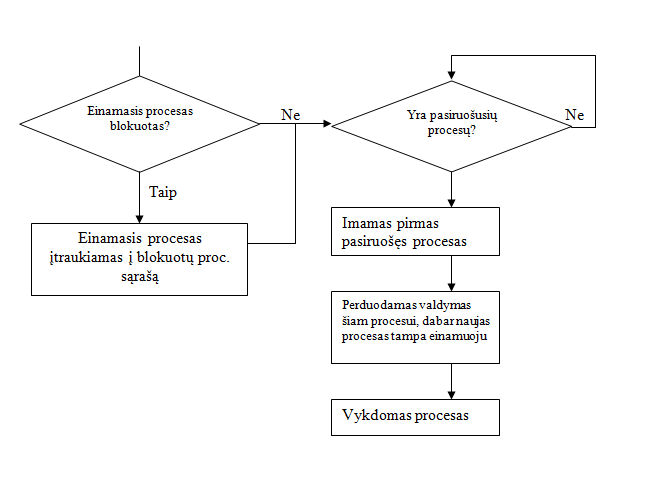
\includegraphics{img/processPlanner.png}

\subsubsection{Procesų primityvai}
Procesų primityvų paskirtis - pateikti vienodą ir paprastą vartotojo sąsają darbui su procesais. Kiekvieno primityvo programos gale yra kviečiamas planuotojas. Yra 4 primityvai:
	\begin{itemize}
		\item Kurti procesą - primityvui perduodama nuoroda į jo tėvą, jo pradinė būsena, prioritetas, perduodamų elementų sąrašas ir išorinis vardas.
			Tada procesas yra registruojamas bendrame procesų sąraše, tėvo sūnų sąraše, skaičiuojamas vidinis identifikacijos numeris.
		\item Naikinti procesą - pradedama naikinti proceso sukurtus resursus ir vaikus. Vėliau procesas panaikinamas iš tėvo procesų sąrašo. Po to iš bendro procesų sąrašo, galiausiai
			naikinami visi jam perduoti resursai ir proceso deskriptorius yra sunaikinamas.
		\item Stabdyti procesą - proceso būsena iš blokuotos keičiama į blokuotą-sustabdytą arba į pasiruošusią-sustabdytą. Einamasis procesas tampa pasiruošusiu-sustabdytu.
		\item Aktyvuoti procesą - keičiama proceso būsena iš blokuotos-sustabdyto į blokuotą arba pasiruošusios-sustabdytos į pasiruošusią.
	\end{itemize}

\subsection{Resursai}
Resursas yra tai, dėl ko varžosi procesai. Dėl resursų trūkumo procesai blokuojasi, gavę reikiamą resursą tampa pasiruošusiais. 

\subsubsection{Resursų deskriptoriai}
\begin{itemize}
	\item RId  – resurso vidinis vardas
	\item RidI – resurso išorinis vardas.
	\item RCreator – nuoroda į procesą sukūrusį šį resursą
	\item RElements – nuoroda i resurso elementu sąrašą
	\item RWaitingProc – nuoroda i resurso laukiančių procesų sąrašą
	\item RWaitingCount – nuoroda i šio resurso laukiančių procesų paprašytų resurso kiekių sąrašą
	\item RLinkList – nuoroda į visų resursų sąrašą
	\item RWaitingProcPoint – nuoroda į šio resurso laukiančių procesų resurso elemento rodyklių sąrašą
	\item RTxt – resurso požymis
\end{itemize}

\subsubsection{Resurso primityvai}
	\begin{itemize}
		\item Kurti resursą \\ Resursus kuria tik procesas. Resurso kūrimo metu perduodami kaip parametrai: nuoroda į proceso kūrėją, resurso išorinis vardas. Resursas kūrimo metu yra: pridedamas prie bendro resursų sąrašo, pridedamas prie tėvo suskurtų resursų sąrašo, jam priskiriamas unikalus vidinis vardas, sukuriamas resurso elementų sąrašas ir sukuriamas laukiančių procesų sąrašas.
		\item Naikinti resursą \\ Resurso deskriptorius išmetamas iš jo tėvo sukurtų resursų sąrašo, naikinamas jo elementų sąrašas, atblokuojami procesai, laukiantys šio resurso, išmetamas iš bendro resursų sąrašo, ir, galiausiai naikinamas pats deskriptorius. 
		\item Prašyti resurso \\Šį primityvą kartu su primityvu “atlaisvinti resursą” procesai naudoja labai dažnai. Procesas, iškvietęs šį primityvą, yra užblokuojamas ir įtraukiamas į to resurso laukiančių procesų sąrašą. Sekantis šio primityvo žingsnis yra kviesti resurso paskirstytoją.
		\item Atlaisvinti resursą \\Šį primityvą kviečia procesas, kuris nori atlaisvinti jam nereikalingą resursą arba tiesiog perduoti pranešimą ar informaciją kitam procesui. Resurso elementas, primityvui perduotas kaip funkcijos parametras, yra pridedamas prie resurso elementų sąrašo. Šio primityvo pabaigoje yra kviečiamas resursų paskirstytojas.
	\end{itemize}

\subsubsection{Resurso paskirstytojas}
Kaip kad procesorius yra skirstomas planuotojo, kiekvienas resursas taipogi yra skirstomas tarn tikro paskirstytojo. Prašydamas resurso ar norėdamas jį atlaisvinti, procesas kreipiasi į atitinkama. resursų paskirstytojo kuris privalo jį aptarnauti.
Resursų paskirstytojo paskirtis - suteikti paprašyta. resurso elementų kiekį procesui. Resursų paskirstytojo algoritmas gali būti sudėtingas. Pavyzdžiui, turi būti numatyta galimybė atiduoti resurso elementą konkrečiam procesui, arba prašyti kelių resurso elementų. Resurso paskirstytojas peržvelgia visus laukiančius šio resurso procesų sajašą, ir, sutikęs galimybę aptarnauti process perduoda jam reikalingus resurso elementus ir pažymi jį pasiruošusiu. Paskirstytojo pabaigoje yra iškviečiamas planuotojas.


\subsubsection{Bazinių procesų paketas}
Mūsų modelyje bus naudojami šie procesai:
	\begin{itemize}
		\item StartStop – šakninis procesas, sukuriantis bei naikinantis sisteminius procesus ir resursus;
		\item ReadFromKey – programos nuskaitymas ir kopijavimas į supervizorinę atmintį;
		\item MainProc – procesas, valdantis JobGovernor procesus;
		\item JobGovernor – virtualios mašinos proceso tėvas, valdantis virtualios mašinos proceso darbą;
		\item VirtualMachine – procesas, atsakantis už vartotojiškos programos vykdymą;
		\item Interrupt – procesas, apdorojantis virtualios mašinos pertraukimą sukėlusią situaciją;
		\item PrintLine – į išvedimo įrenginį persiunčiamas blokas iš vartotojo atminties;
		\item GetLine – iš įvedimo įrenginio nuskaitomas blokas į vartotojo atminties.
		\item Memory Governor - valdo bendrąją atmintį.
	\end{itemize}
Visi procesai, išskyrus VirtualMachine (šį procesą sukuria JobGovernor) ir JobGovernor, yra sukuriami sistemos darbo pradžioje proceso StartStop.

\subsection{Procesų aprašai}

\subsubsection{Procesas StartStop}
Šis procesas atsakingas už sistemos darbo pradžią ir pabaigą. Įjungus komputerį (paleidus MOS modelį), šis procesas pasileidžia automatiškai. Šio proceso paskirtis, sisteminių procesų bei resursų kūrimas.

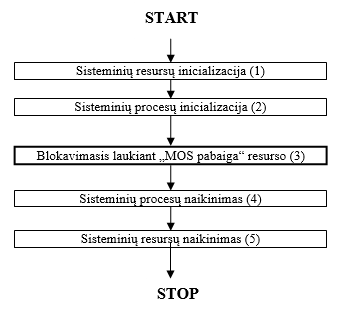
\includegraphics{img/StartStop.png}

	\begin{itemize}
		\item Procesas, gavęs procesorių, savo darbą pradeda sukurdamas visus sisteminius resursus (1). 
		\item Sukūręs resursus, procesas kuria nuolatinius procesus (2), t.y. tokius procesus, kurie bus aktyvūs visą MOS gyvavimo laiką (visi, išskyrus JobGovernor ir VirtualMachine).
		\item Prašo resurso „MOS pabaiga“ (3), t.y. šioje vietoje procesas blokuojasi ir laukia, kol bus atlaisvintas pranešimas apie MOS darbo pabaigą. Priklausomai nuo prioriteto šis procesas bus atblokuotas ir tęs darbą.
		\item Visų sisteminių procesų naikinimas (4). 
		\item Sisteminių resursų naikinimas (5). MOS darbo pabaiga.
	\end{itemize}
\subsubsection{Procesas ReadFromKey}
Šį procesą kuria ir naikina procesas StartStop. Šio proceso paskirtis – gavus informaciją iš įvedimo srauto, atiduoti informaciją tolesniam apdorojimui, kurį atliks procesas MainProc.

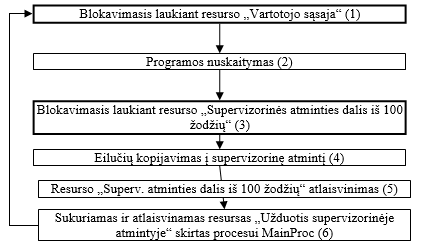
\includegraphics{img/ReadFromKey.png}

	\begin{itemize}
		\item Pirmasis žingsnis – laukti įvedimo srauto (1).  Įvedimo srautu ateina programos tekstas.
		\item Programos teksto nuskaitymas (2).
		\item Prašome resurso „Supervizorinės atminties dalis iš 100 žodžių“ (3) ir kopijuojame eilutes į supervizorinę atmintį (4).
		\item Atlaisviname resursą „Supervizorinės atminties dalis iš 100 žodžių“ (5).
		\item Sukuriamas ir atlaisvinamas resursas, skirtas procesui MainProc, su komponente „Vykdyti“, lygia 1. (6). 
		\item Proceso programa yra ciklinė, todėl ReadFromKey vėl užsiblokuoja laukdamas.
	\end{itemize}
\subsubsection{Procesas MainProc}
Šio proceso paskirtis – kurti ir naikinti procesus JobGovernor.

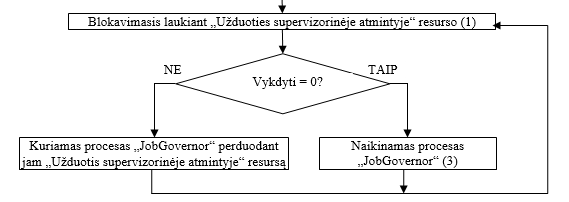
\includegraphics{img/MainProc.png}

	\begin{itemize}
		\item Procesas prašo užduoties („Užduotis supervizorinėje atmintyje“ resursas, kurį atlaisvina procesas ReadFromKey), kurią reikia įvykdyti (1).
		\item Tikrinama, ar resurso komponentė „Vykdyti“ lygi 0, t.y. ar užduotis jau baigta vykdyti.
		\item Jei Vykdyti nelygus nuliui, kuriamas procesas „JobGovernor“, priešingu atveju naikinamas procesas „JobGovernor“. (2, 3).
		\item Atlikęs savo darbą, procesas MainProc vėl blokuojasi laukdamas resurso (1).
	\end{itemize}
\subsubsection{Procesas JobGovernor}
Procesus JobGovernor kuria procesas MainProc. Šių procesų paskirtis – padėti procesui VirtualMachine atlikti savo darbą (atlikti veiksmus, kurių virtuali mašina procesoriui dirbant vartotojo režimu nesugeba atlikti).

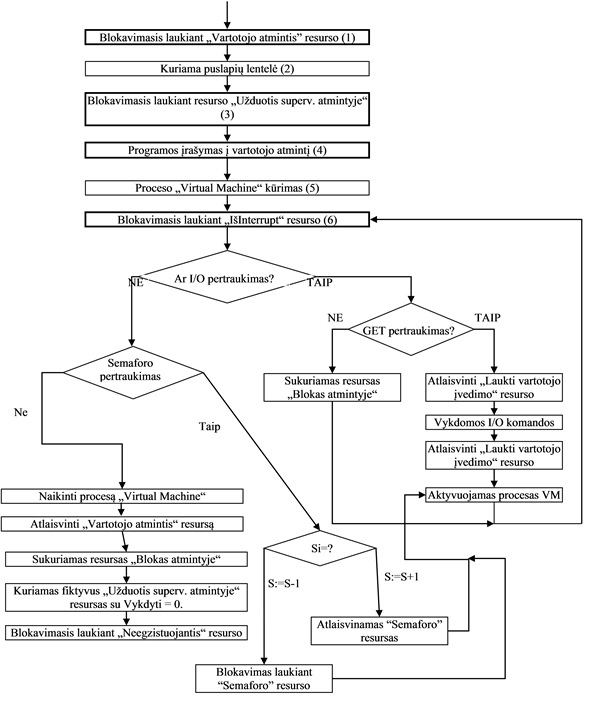
\includegraphics{img/JobGovernor.jpg}

	\begin{itemize}
		\item Procesas prašo vartotojo atminties, kad galėtų patalpinti vartotojo užduoties programą. Sukuriama puslapių lentelė ir užpildoma išskirtos vartotojo atminties adresais. Perkėlus vartotojo užduoties programą į vartotojo atmintį, programa pašalinama iš supervizorinės atminties (1, 2, 3, 4). 
		\item Kuriama virtuali mašina, t.y. procesas VirtualMachine (5).
		\item Procesas JobGovernor blokuojasi ir laukia pertraukimo proceso VirtualMachine vykdymo metu (6).
		\item Gavus pranešimą apie pertraukimą (pertraukimai gali kilti, kai TI=0 arba vykdomos komandos GET, PUT, HALT), tikrinama, ar tai įvedimo/išvedimo pertraukimas (7).
		\item Jei tai nėra įvedimo/išvedimo pertraukimas, naikinamas procesas VirtualMachine, atlaisvinama virtualios mašinos užimta vartotojo atmintis. Sukuriamas resursas „Blokas atmintyje“ užduoties vykdymo statistikai išvesti. Kuriamas ir atlaisvinamas fiktyvus resursas „Užduotis superv. atmintyje“ su komponente Vykdyti = 0, skirtas procesui MainProc (tai požymis, kad šis JobGovernor baigė savo darbą ir turi būti sunaikintas). Kol šis JobGovernor procesas nėra sunaikintas (nors jau baigė darbą), jis blokuojasi laukdamas „Neegzistuojantis“ resurso. Kadangi šio resurso jis negaus, procesas blokuosis, kol bus galiausiai sunaikintas.
		\item Jei tai GET pertraukimas, sukuriamas resursas „Laukti vartotojo įvedimo“ (skirtas procesui GetLine), su komponente, nurodančia, kur rašyti duomenis ir kokiam procesui „VirtualMachine“ sukurti pranešimą apie baigtą procesą.
		\item Jei tai PUT pertraukimas, sukuriamas resursas „Blokas atmintyje“ su komponente, nurodančia, kur rašyti duomenis ir kokiam procesui „VirtualMachine“ sukurti pranešimą apie baigtą procesą.
	\end{itemize}
\subsubsection{Procesas VirtualMachine}
Procesą kuria ir naikina procesas JobGovernor. Proceso VirtualMachine paskirtis yra vykdyti vartotojo užduoties programą. Šių procesų yra tiek, kiek yra procesų JobGovernor.

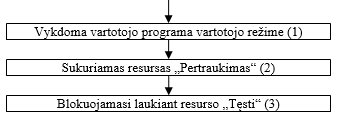
\includegraphics{img/VirtualMachine.png}

	\begin{itemize}
		\item Interpretuojama programa, kol neįvyksta pertraukimas (1).
		\item Įvykus pertraukimui, virtuali mašina išsaugo savo procesoriaus būseną, valdymas perduodamas pertraukimą apdorosiančioms programoms. Kuriamas resursas „Pertraukimas“ skirtas procesui Interrupt, kuris indentifikuos pertraukimą ir perduos informaciją procesui JobGovernor (2), ir laukiama leidimo tęsti vykdymą (pranešimo apie įvykdytą veiksmą iš įvedimo/išvedimo procesų).
	\end{itemize}
\subsubsection{Procesas Interrupt}
Procesą Interrupt kuria ir naikina procesas StartStop. Šio proceso paskirtis – reaguoti į pertraukimus, kilusius virtualios mašinos darbo metu. 

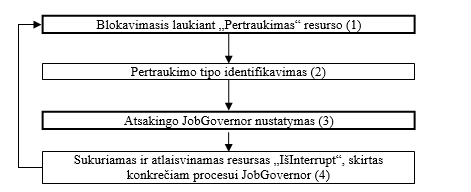
\includegraphics{img/Interrupt.png}

	\begin{itemize}
		\item Procesas Interrupt savo darbo pradžioje laukia „Pertraukimas“ resurso, kurį siunčia procesas VirtualMachine (1).
		\item  Procesas nustato pertraukimo tipą apklausinėdamas pertraukimo programų nustatytas sisteminių kintamųjų reikšmes (2).
		\item Toliau procesas cikliškai blokuojasi vėl laukdamas „Pertraukimas“ resurso. Kiekviena virtuali mašina kūrimo metu laiko savo tėvo JobGovernor identifikatorių. Kartu su pranešimu apie pertraukimą yra perduodamas ir tas identifikatorius, kurį Interrupt naudoja jam reikalingo JobGovernor atskyrimui iš kitų (3).
		\item Galiausiai yra kuriamas ir atlaisvinamas „IšInterrupt“ resursas, kuris yra skirtas nustatytajam JobGovernor procesui (4). 
	\end{itemize}
\subsubsection{Procesas PrintLine}
Procesą PrintLine kuria ir naikina procesas StartStop. Šio proceso paskirtis – į išvedimo srautą pasiųsti pranešimą
	
\subsubsection{Procesas GetLine}
Procesą GetLine kuria ir naikina procesas StartStop. Šio proceso paskirtis – iš įvedimo srauto nuskaityti duomenis. 

\subsubsection{Procesas Memory Governor}

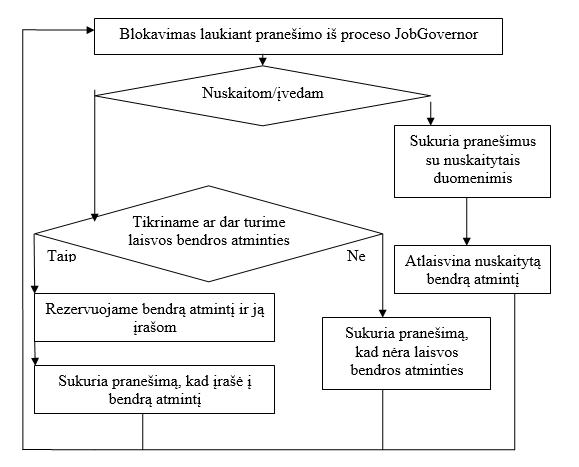
\includegraphics{img/MemoryGovernor.png}

MemoryGovernor - procesas valdantis bendrąją atmintį. Norint naudotis bendra atmintimi, reikia kreiptis į GenMemory procesą ir laukti atsakymo ar galima naudotis prašomu bendros atminties bloku.
\subsection{Samaforai}

Semaforas S tai sveikas neneigiamas skaičius, su kuriuo atliekamos operacijos P(S) ir V(S), kur P ir V nauji primityvai. Operacijos pasižymi savybėmis:
\begin{itemize}
	\item P(S), V(S) – nedalomos operacijos, t.y. jų valdymo negalima pertraukti ir jų vykdymo metu negalima kreiptis į semaforą S;
	\item V(S):     S:S+1; (didinama semaforo reikšmė)
	\item P(S):      S:S-1; (sumažinama jei S>0)
	\item Jei S=0, tai procesas P, kuris vykdo operaciją P(S), laukia, kol sumažinimas vienetu bus galimas. Šiuo atvėju P(S) yra pertraukiamas
	\item Jei keletas procesų vienu metu iškviečia V(S) ir/ar P(S) su vienu semaforu, tai užklausimai vykdomi nuosekliai, kokia nors iš anksto nežinoma tvarka.
	\item Jei keletas procesų laukia operacijos P(S) įvykdymo, S – ta pats, tai reikšmei tapus teigiamai (kai kažkuris procesas įvykdė operaciją V(S)), kažkuris iš laukiančių procesų bus pradėtas vykdyti.
Pagal prasmę operacija P atitinka perėjimo išškvietimą, o V – kito proceso aktyvaciją.
\end{itemize}
